\section{Geschäftsidee}


\subsection{Womit wir uns befassen}
Eine Studie von International Data Corporation (IDC, eines der führenden Marktforschungsunternehmen in der IT-Industrie) aus dem Jahr 2005\footnote[1]{\textit{White Paper on Hidden Cost of Information Work}, IDC, 2005.} hat gezeigt, dass ein Wissensarbeiter im Durchschnitt rund ein Viertel seiner Arbeitszeit alleine auf die Informationssuche aufwendet. In der wissenschaftlichen Forschung ist dieser Anteil unseren Schätzungen zufolge noch größer. Gesucht wird dabei vor allem nach Information in Form von wissenschaftlichen Publikationen. Weil Publikationen im Idealfall den Stand der Technik abbilden, ist deren Studium ein Grundpfeiler erfolgreicher wissenschaftlicher Praxis. 

\begin{table}[h!]
  \centering
  \begin{large}
	\begin{itshape}
  \begin{tabular}{c}\hline
	\\
  {\color{orange}„Wenn ich weiter geblickt habe, so deshalb,} \\ 
	{\color{orange}weil ich auf den Schultern von Riesen stehe.“} \\
	{\hfill \color{orange}\textit{Isaac Newton, 1676} } \\
	\\\hline
  \end{tabular}
	\end{itshape}
  \end{large}
\end{table}

Neben den obligatorischen Veröffentlichungen in Journals und Konferenzbändern bergen Blogs und Magazine häufig eine nicht minder wichtige Quelle für neue Ideen und Herangehensweisen. An dieser Stelle kommen allerdings vier wichtige Faktoren ins Spiel, die eine erfolgreiche Literaturrecherche erheblich erschweren: 

\begin{description}
  \item[\textbf{\color{orange}{Informationsuniversum wächst:}}] \hfill \\
  Die Zahl möglicher Quellen und potentiell wertvoller Informations-Items wächst rasant: 
In 2008 erschienen allein in den neun\footnote[2]{Nach UNESCO Science Report 2010: GER, FRA, UK, RUS, JPN, KOR, CHN, CAN, USA} großen Wissenschaftsnationen 760.671 Veröffentlichung. Bei der gegenwärtigen jährlichen Wachstumsrate von 3,26\% wird sich diese Zahl in zwanzig Jahren verdoppeln. 
  \item[\textbf{\color{orange}{Information veraltet:}}] \hfill \\
  Neu produziertes Wissen veraltet heute schneller als jemals zuvor. Neue Entwicklungen in einem Forschungsfeld werden schnell entdeckt, aufgegriffen und weiterentwickelt. Wenn man Fortschritt erzielen möchte, ist jede Verzögerung bei der Informationssuche ein schwerwiegender Nachteil. 
  \item[\textbf{\color{orange}{Wissensgebiete werden vernetzt:}}] \hfill \\
  Die Grenzen zwischen den Disziplinen verschwimmen zunehmend. Bahnbrechende Arbeiten über Datenverarbeitung werden manchmal in Biologie-Journals publiziert, weil beispielsweise die Genomforschung ohne Informatik nicht mehr auskommt. Solche potentiell interessanten Informations-Events bleiben natürlich unentdeckt, wenn man die Aufmerksamkeit unmittelbar auf das eigene Feld beschränkt. 
 \item[\textbf{\color{orange}{Verfügbare Such-Tools sind unzulänglich:}}] \hfill \\
	Die Möglichkeiten der Suche in der globalen Informationswolke, bereitgestellt durch Incumbents wie Google und Microsoft, sind weitgehend auf Schlüselworte beschränkt. Dabei ist die Suche nach Bedeutungs-Nuancen und Konzepten das, was eine effektive Literaturrechere ausmacht. 
\end{description} Diese Probleme wird \textsc{\color{orange}{SemLit}} lösen. Mit semantischen Technologien werden wir die Praxis der Literaturarbeit umkrempeln. Im Folgenden beschreiben wir, wie das im Detail geschehen soll. 

\begin{table}[h!]
  \centering
  \begin{large}
	\begin{itshape}
  \begin{tabular}{c}\hline
  \\
  {\color{orange}Ein Wissensarbeiter verbringt durchschnittlich }\\
  {\color{orange}24\% seiner Zeit mit Informationssuche.}\\
  \\\hline
  \end{tabular}
	\end{itshape}
  \end{large}
\end{table}


%=======================================

\subsection{Know-how Träger}
Die Idee und Umsetzung wird von zwei Studenten des Karlsruher Instituts für Technologie (KIT) entwickelt. {\color{orange}Artem Schumilin} studiert Wirtschaftsingenieurwesen (M.Sc) und {\color{orange}Igor Tseyzer} studiert Informationswirtschaft (B.Sc). Wahrend des Studiums am KIT haben beide Gründer die notwendigen Kenntnisse in Web- und Semantic-Web-Technologien gesammelt, was als stabiles Fundament für den Aufbau und weitere Entwicklung der Firma dienen soll. 
\begin{figure}[h!]
\centering

\includegraphics[width=0.6\textwidth]{jsi-aifb-logo}
\end{figure}

Außerdem stehen den Gründern renommierte Partner aus der Forschung zur Seite: 
Das Josef-Stefan-Institut (JSI) hat mit Enrycher die weltweit führende \emph{named entity recognition engine} entwickelt und tritt damit als der Tchnologiepartner von SemLit auf. 
Das Institut AIFB des KIT erweist sich erfahrener Mentor in Sachen Ausgründung im Bereich semantischer Technologie und wird das Start-Up mit seinen Kontakten und Rat unterstützen.

%=======================================

\subsection{Innovation}

\textsc{Schritt 0:} wo es beginnt\\
Wir beginnen bei den Informations-Items, die im Internet zur freien Verfügung stehen. Dazu gehören vor allem die Abstracts von wissenschaftlichen Veröffentlichungen aus Journals und Konferenzbänden aber auch Artikel in relevanten Blogs und Online-Magazinen. Die Vielzahl der Quellen wird automatish überwacht, um die Nahezu-Echtzeit-Anforderung erfüllen zu können.\\
{\color{orange}Unsere Kunden können die Auswahl der Quellen auf ihre individuellen Bedürfnisse anpassen. }
\\
\\
\textsc{Schritt 1:} die Semantik hinter dem Text\\
Der Kerngedanke hinter SemLit gründet auf den Möglichkeiten, die durch semantische Repräsentation von Textinformation entehen. Dazu gehört die Erkennung von named entities und ihrer Beziehungen untereinander. Mit JSI's Enrycher steht uns die derzeit weltbeste Technologie bereit, mit deren Hilfe wir die Extraktion semantischer Information aus Textdokumenten realisieren. 
\\
\\
\textsc{Schritt 2: Informationswunsch äußern}\\
Wie die Textinformation auf der einen Seite, können auf der anderen Seite auch die Suchanfrage der Kunden semantisch repräsentiert werden. Damit kann der Benutzer extrem nuancierte Konzepte ausdrücken. 
Dieses semantische \emph{information retrieval} liefert deutlich bessere Ergebnisse als die gewöhnliche Schlüsselwortsuche alleine. Schlüsselworte sind oft mehrdeutig und liefern damit irrelevante Suchergebnisse, die unnötig Zeit kosten. \\
{\color{orange}Bei SemLit sucht der Benutzer nicht nach einem Wort, sondern nach dem Sinn, der hinter diesem Wort steckt.}
\\
\\
\textsc{Schritt 3: wir gehen weiter als die Anderen}\\
Wir bleiben keineswegs bei den Suchanfragen stehen, sondern gehen noch einen Schritt weiter: Nichts sagt mehr über das Suchinteresse eines Benutzers aus als seine bestehende Dokumentsammlung. Warum also nicht daraus lernen? --- Bei SemLit hat der Kunde die Möglichkeit, ein individuelles System durch Hochladen eigener Dokumente zu trainieren.
\\
\\
{\color{orange}Unter dem Strich entsteht eine Webplattform zur automatischen und individuellen Überwachung der Informationslandschaft. Das System weiß, was der Benutzer will und informiert ihn rechtzeitig, wenn die passende Publikation, der Blogeintrag oder News-Artikel in Web auftaucht.}


\begin{figure}[h!]
\centering
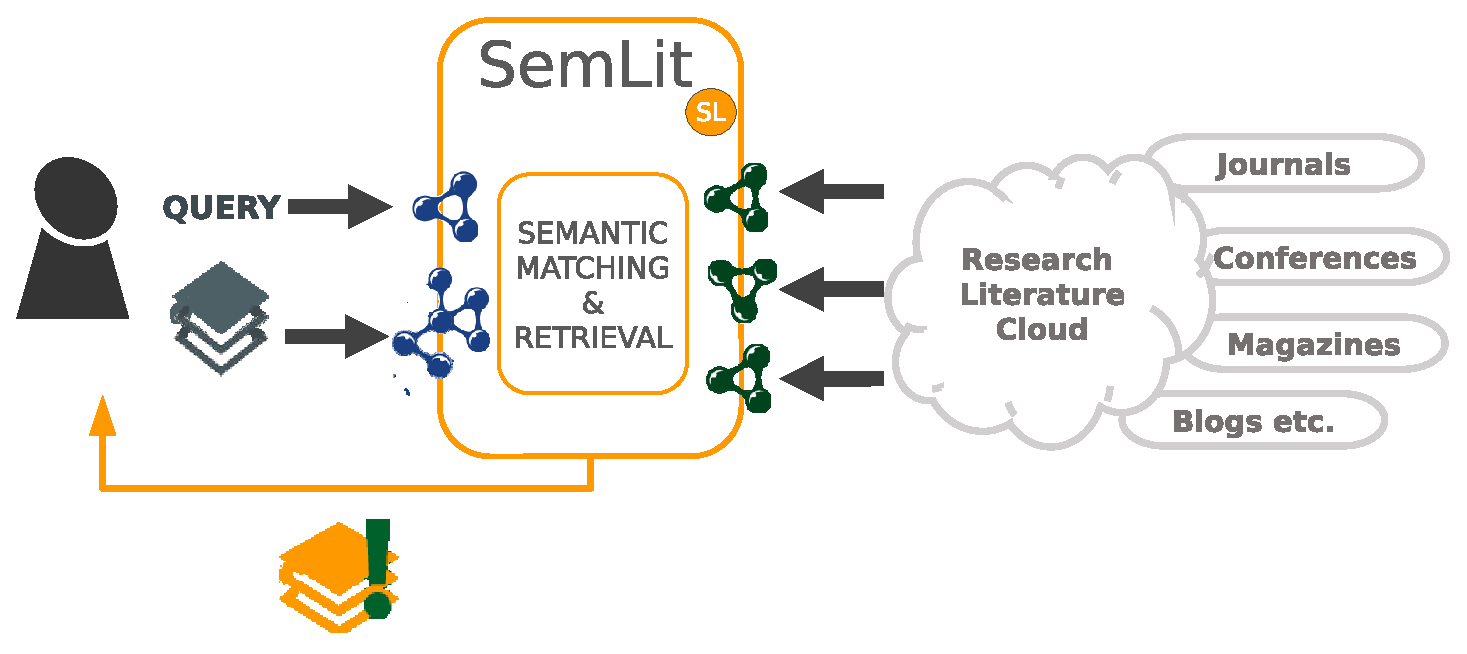
\includegraphics[width=0.9\textwidth]{idea}
\caption{Funktionsschema von SemLit}
\label{fig:idea}
\end{figure}


%=======================================

\subsection{Projektplanung}

SemLit ist in zwei Formen verfügbar: Webauftritt und App für Mobile Geräte. Das Mockup für Webauftritt und Mobile APP können in Abbildung \ref{fig:web} und \ref{fig:app} gesehen werden.

\begin{figure}[h!]
\centering
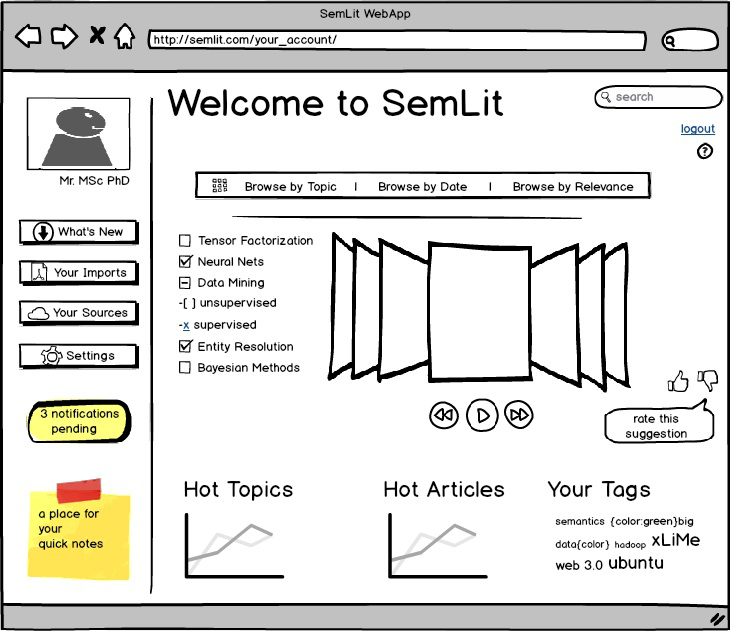
\includegraphics[width=0.6\textwidth]{mockup_web}
\caption{Mockup für Webauftritt}
\label{fig:web}
\end{figure}

\begin{figure}[h!]
\centering
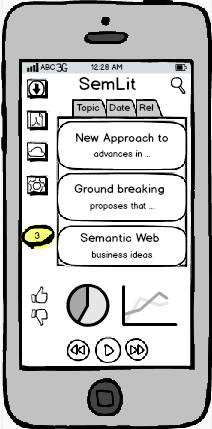
\includegraphics[width=0.2\textwidth]{mockup_app}
\caption{Mockup für Mobile App}
\label{fig:app}
\end{figure}

Die Beide Formen sind Benutzer freundlich und stellen eine Möglichkeit schnell und ohne zusätzliche Aufwand gewünschte Information suchen und verwalten.\\


